
% disjoint_injective.tex
% Illustrates that disjoint injective embeddings preserve representability:
% a collection of per-type functions {f_j} can be replicated by a single
% function f over the shared domain.
%
% Usage: \includegraphics[width=\linewidth]{disjoint_injective.tex}
%   (via tikzscale, which is already loaded in the defense preamble)

\documentclass[tikz]{standalone}
\usepackage{amsmath,amssymb}
\usetikzlibrary{positioning, arrows.meta, decorations.pathmorphing, fit, calc}

\begin{document}
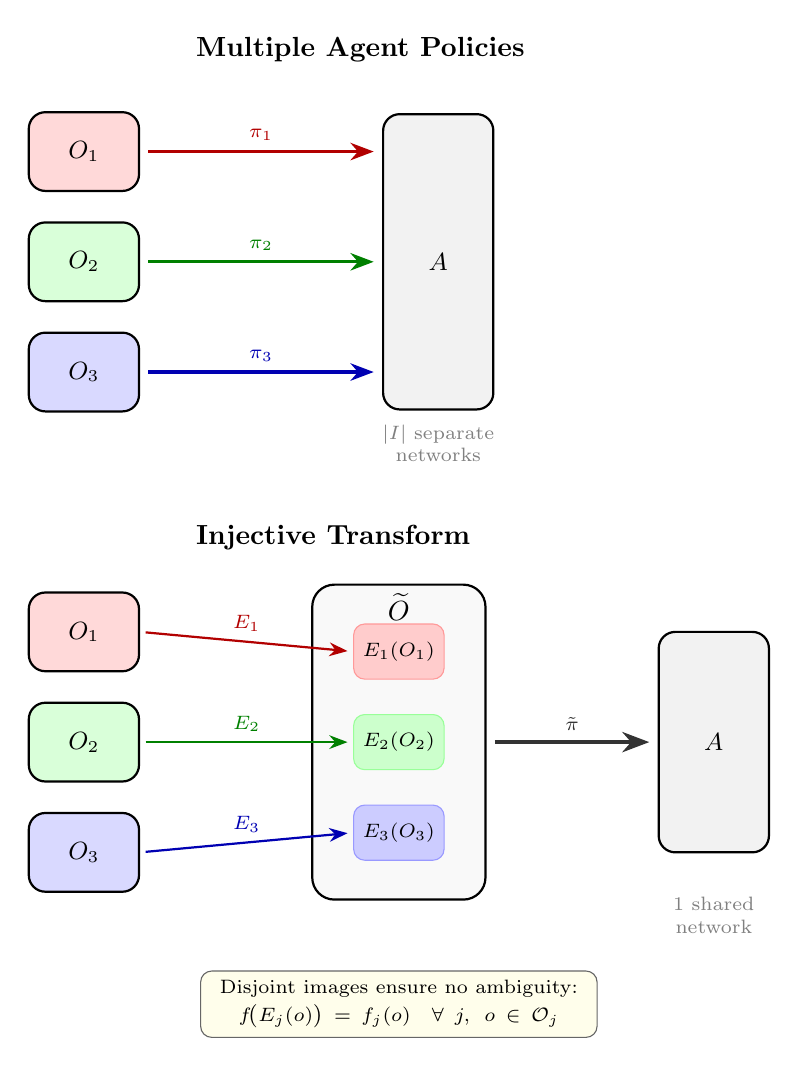
\begin{tikzpicture}[
    >=Stealth,
    every node/.style={font=\small},
    space/.style={
        draw, rounded corners=6pt, minimum width=1.4cm, minimum height=1.0cm,
        thick, align=center
    },
    bigspace/.style={
        draw, rounded corners=8pt, thick, inner sep=8pt, align=center
    },
    region/.style={
        rounded corners=4pt, minimum width=1.1cm, minimum height=0.7cm,
        align=center, font=\scriptsize
    },
    mapsto/.style={->, thick, shorten >=2pt, shorten <=2pt},
    funcline/.style={->, very thick, shorten >=3pt, shorten <=3pt},
    dashedfunc/.style={->, thick, densely dashed, shorten >=3pt, shorten <=3pt},
]

% =====================================================================
%  TOP ROW:  Per-type functions  {f_j : O_j -> Y}
% =====================================================================
\node[font=\normalsize\bfseries, anchor=west] at (1.3, 3.5)
    {Multiple Agent Policies};

% Input spaces
\node[space, fill=red!15]   (O1) at (0, 2.2) {${O}_1$};
\node[space, fill=green!15]  (O2) at (0, 0.8) {${O}_2$};
\node[space, fill=blue!15]  (O3) at (0,-0.6) {${O}_3$};

% Output space (top)
\node[space, fill=gray!10, minimum height=3.75cm] (Y1) at (4.5, 0.8) {$A$};

% Per-type function arrows
\draw[funcline, red!70!black]   (O1.east) -- node[above, font=\scriptsize] {$\pi_1$} (Y1.west |- O1);
\draw[funcline, green!50!black] (O2.east) -- node[above, font=\scriptsize] {$\pi_2$} (Y1.west |- O2);
\draw[funcline, blue!70!black]  (O3.east) -- node[above, font=\scriptsize] {$\pi_3$} (Y1.west |- O3);

% Brace / annotation
\node[font=\scriptsize, text=gray, align=center] at (4.5, -1.5)
    {$|{I}|$ separate\\networks};

% =====================================================================
%  BOTTOM ROW:  Single function  f : \tilde{O} -> Y
% =====================================================================
\node[font=\normalsize\bfseries, anchor=west] at (1.3, -2.7)
    {Injective Transform};

% Input spaces (repeated, lower)
\node[space, fill=red!15]   (O1b) at (0, -3.9) {${O}_1$};
\node[space, fill=green!15]  (O2b) at (0, -5.3) {${O}_2$};
\node[space, fill=blue!15]  (O3b) at (0, -6.7) {${O}_3$};

% Homogenized space with disjoint regions
\node[bigspace, fill=gray!5, minimum width=2.2cm, minimum height=4.0cm]
    (Otilde) at (4.0, -5.3) {};
\node[font=\normalsize, anchor=north] at (Otilde.north) {$\widetilde{{O}}$};

% Disjoint embedded regions inside Otilde
\node[region, fill=red!20,   draw=red!40]   (R1) at (4.0, -4.15) {$E_1({O}_1)$};
\node[region, fill=green!20,  draw=green!40] (R2) at (4.0, -5.30) {$E_2({O}_2)$};
\node[region, fill=blue!20,  draw=blue!40]  (R3) at (4.0, -6.45) {$E_3({O}_3)$};

% Embedding arrows
\draw[mapsto, red!70!black]   (O1b.east) -- node[above, font=\scriptsize] {$E_1$} (R1.west);
\draw[mapsto, green!50!black] (O2b.east) -- node[above, font=\scriptsize] {$E_2$} (R2.west);
\draw[mapsto, blue!70!black]  (O3b.east) -- node[above, font=\scriptsize] {$E_3$} (R3.west);

% Output space (bottom)
\node[space, fill=gray!10, minimum height=2.8cm] (Y2) at (8.0, -5.3) {$A$};

% Single function arrow
\draw[funcline, black!80, line width=1.5pt]
    (Otilde.east) -- node[above, font=\scriptsize] {$\tilde\pi$} (Y2.west);

% Annotation
\node[font=\scriptsize, text=gray, align=center] at (8.0, -7.5)
    {1 shared\\network};

% =====================================================================
%  KEY PROPERTY annotation
% =====================================================================
\node[draw=black!60, rounded corners=4pt, fill=yellow!8,
      font=\scriptsize, align=center, text width=4.8cm,
      anchor=north] at (4.0, -8.2)
    {Disjoint images ensure no ambiguity:\\[2pt]
     $f\!\bigl(E_j(o)\bigr) = f_j(o)
     \;\;\forall\; j,\; o \in \mathcal{O}_j$};

\end{tikzpicture}
\end{document}